%ब

\section{Solution 1:  Metadata with Special Characters} \label{s:design-sol1}

% \subsection{Metadata Storage}
In this  solution,   metadata is embedded with the actual data and is
stored in the column family of the actual data.  In this approach,  metadata is
stored in every super column of a column family  as the value of column
\texttt{Metadata} (Figure~\ref{fd:Metadata-Column}).  Since metadata is
common for all the super columns in a column family,  every super column
contains the same  value in the \texttt{Metadata} column. 
% For example,  in the
% University keyspace,  metadata in \texttt{Student} is  as seen in
Figure~\ref{fd:Metadata-Solution1} presents how metadata is stored in every
super column of the example \texttt{Student} column family in the University
keyspace. 
	
 
		
In this approach,  metadata contains all the parts as 
% the structure of the
% constraints in metadata is as 
described in Section~\ref{s:design-Metadata} and each column family stores only
the constraints relevant to its dependencies.  Thus,  a column family contains
only its \ac{PK} constraint and related \ac{FK} constraints in its
\texttt{Metadata} column.  The following are the types of constraints stored in
each of the column families. 
	
		\begin{itemize}
		  \item  \ac{PK} constraint showing the primary key of the column family. 
		  \item \ac{FK} constraints 
				\begin{itemize}
					\item In the case of a parent column family, the \ac{FK} constraints refer
					to those of type '\texttt{F}' in order to identify the child column
					families.
					\item  In the case of a child column family, the \ac{FK} constraints of
					type '\texttt{R}' are stored to indicate the parent column families. 
					\item If a column family is both a parent and a child,  then its metadata
					stores its \ac{PK} constraint and the \ac{FK} constraints of both types to
					indicate its parent and child column families. For example, if
					\texttt{Enrolment} had a child dependency, it will be a parent to
					that child column family whilst it is also a child of \texttt{Student} and
					\texttt{Course} column families. Its metadata will contain its \ac{PK}
					constraint and \ac{FK} constraints of types '\texttt{R}' and '\texttt{F}'.
				\end{itemize}
		\end{itemize}
		

For instance,  \texttt{Student}  is a parent column family with
\texttt{Enrolment} as its child column family. 
Thus,  its metadata  contains its \ac{PK} constraint \texttt{CONST100} and
the \ac{FK} constraint \texttt{CONST700}.  Since \texttt{Enrolment} is a child entity
it  stores its \ac{PK} constraint \texttt{CONST300} and its \ac{FK} constraints
\texttt{CONST400} and \texttt{CONST500}.  Similarly,  other entities like
\texttt{Course} store its \ac{PK} and respective \ac{FK} constraints. 

	\begin{figure}[h] 
			\centering
				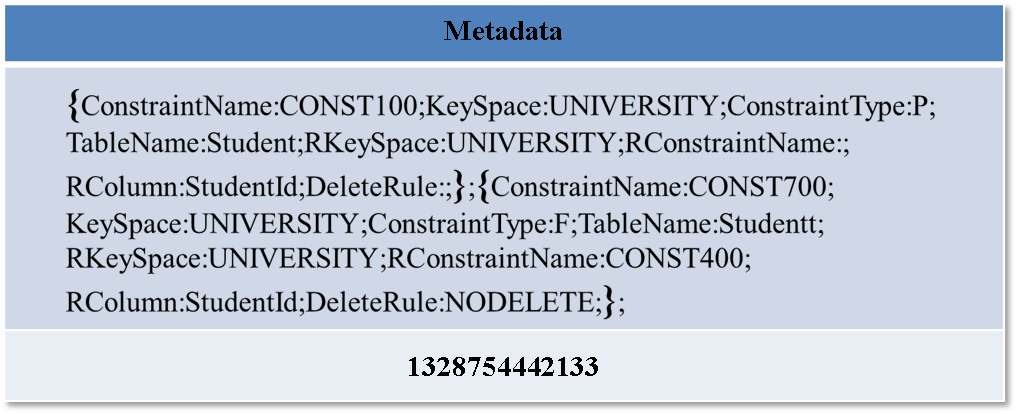
\includegraphics[width=.8\textwidth]{./figure/Solutions/Sol1-MD-Col.png}
				\caption{Metadata Column in Solution 1}
				\label{fd:Metadata-Column}
	\end{figure}
	
	\begin{sidewaysfigure}
		\begin{landscape}
			\centering
			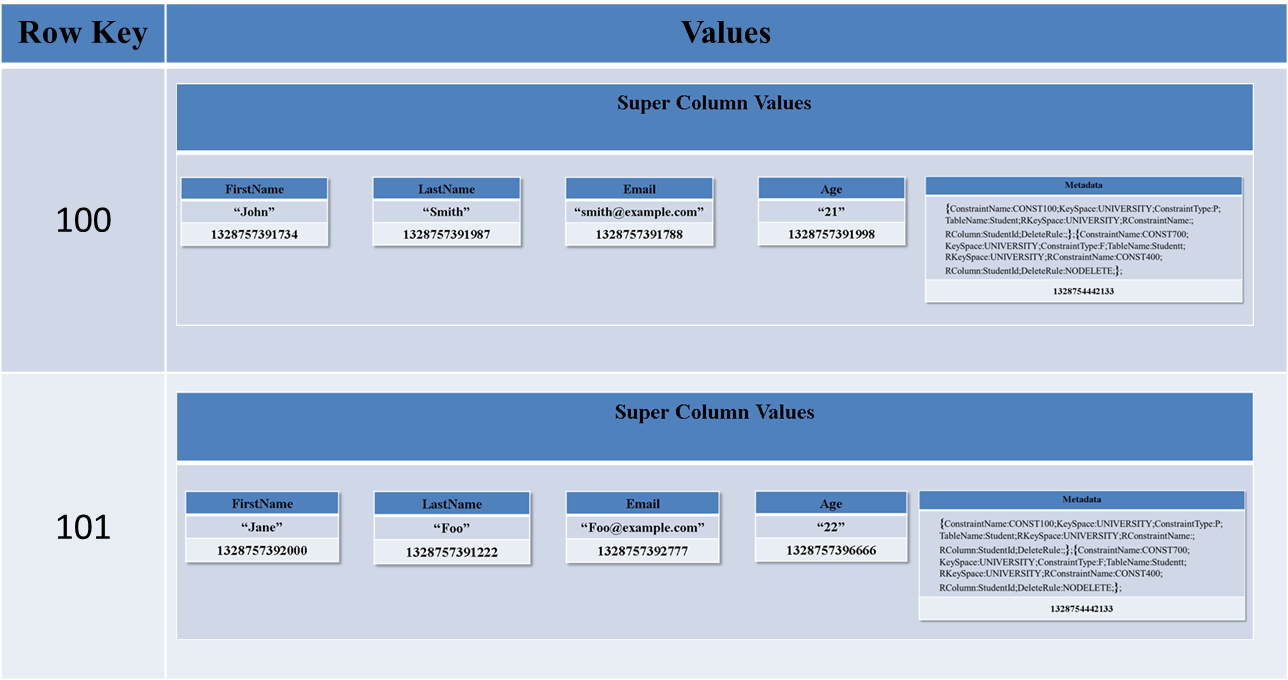
\includegraphics[width=1\textwidth]{./figure/Solutions/Sol1-MD-ColumnFamily.png}
			
			\caption{Metadata in Solution 1}\label{fd:Metadata-Solution1}
			\end{landscape}
		\end{sidewaysfigure}
	
% 	
% 		\begin{figure}[h] \label{fd:Metadata-Solution1}
% 			\centering
% 			\subfigure[Metadata Column] {
% 				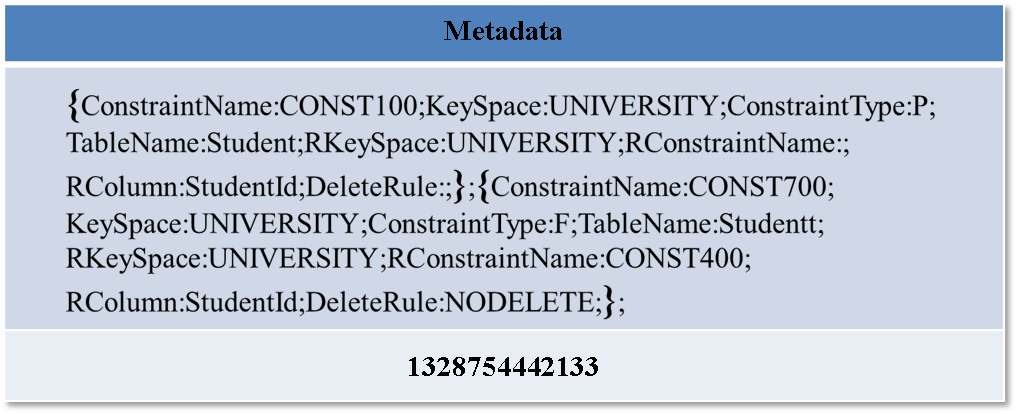
\includegraphics[width=.6\textwidth]{./figure/Solutions/Sol1-MD-Col.png}
% 				\label{fd:Metadata-Solution1-A}
% 	% 			\caption{Response Time for \texttt{insert}}\label{fr:response-insert}
% 			}
% 			\subfigure[Metadata in Super columns]{
% 				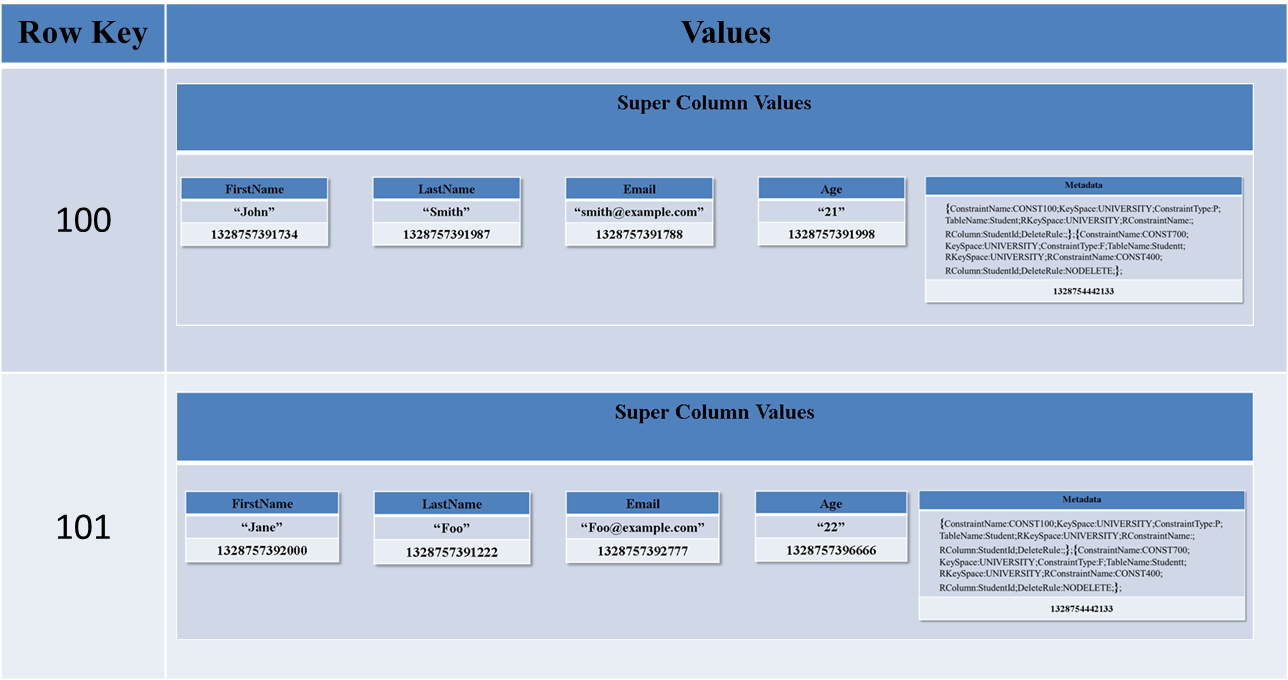
\includegraphics[width=.8\textwidth]{./figure/Solutions/Sol1-MD-ColumnFamily.png}
% 				\label{fd:Metadata-Solution1-B}
% 	% 			\caption{Throughput}\label{fr:through-insert}
% 			} 
% 			\caption{Metadata storage in Solution 1}
% 		\end{figure}
		
Since the relevant constraints of a column family are saved
together in the \texttt{Metadata} column,  it is essential that each constraint
is easily identifiable and accessible.  To separate
the constraints and to identify its different parts, special characters are used
within the metadata as shown in Figure~\ref{fd:Metadata-Column}. These   
characters are curly brackets ('\texttt{\{}', '\texttt{\}}') and
semi-colon and colon ('\texttt{;}', '\texttt{:}'). These special characters are
used as follows. 



% 
% {\setlength{\fboxsep}{6pt}%
% \setlength{\fboxrule}{1pt}%
% 
% \fbox{\parbox{.9\linewidth}{\tt\centering
% % \{ConstraintName:CONST100;KeySpace:UNIVERSITY;ConstraintType:P;\\
% % TableName:Student;RKeySpace:UNIVERSITY;RConstraintName:;\\
% % RColumn:StudentId;DeleteRule:;\};\\
% \{ConstraintName:CONST700;KeySpace:UNIVERSITY;ConstraintType:F;\\
%  TableName:Studentt;RKeySpace:UNIVERSITY;RConstraintName:CONST400;\\
%  RColumn:StudentId;DeleteRule:NODELETE;\};\\
% }}
% }

% \vspace{12pt}

% The special characters :
	
		\begin{itemize}
			\item Each constraint is enclosed in curly brackets and the
			constraints are separated from each other with a
			'\texttt{;}'.  For example, in the \texttt{Student} column
			family,  \texttt{CONST100} and \texttt{CONST700} are enclosed in curly braces
			and separated by '\texttt{;}'. 
			Thus,  '\texttt{\};}' marks the end of every constraint in the metadata. 
		
		
			\item The different parts in a constraint are separated by the special character
			'\texttt{;}'.  For example,  the \texttt{ConstraintName}
			and \texttt{Keyspace} and other parts in the constraints \texttt{CONST100} and
						 \texttt{CONST700} are separated with a '\texttt{;}'. 
			 
			 
			\item Each part and its respective value are separated by the special
			character '\texttt{:}'.  For example,  \texttt{ConstraintName} is separated from
			its value \texttt{CONST100} with a '\texttt{:}'.  
			
		\end{itemize}



		
The special characters help in identifying the values of every constraint in the
metadata information for this solution.  The metadata is extracted from each
super column and processed by specific methods within the solution so that
relevant constraints are used for validating referential integrity.  
% Different
% methods are built in the experimental \ac{API} to support these functionalities
% and these are described in Chapter~\ref{c:Implementation}. 

% In this solution,  the metadata is  repeated several times within the
% same column family and due to the replicated nature of the \ac{NoSQL} \acp{DBMS}
% the metadata is  stored several times across the nodes in the cluster.  This
% increases the redundancy of the metadata and much space would be consumed
% unnecessarily if the metadata is large.  

This design was inspired by the experiments done by (\todo{Hackl et al.  
(2010)}) on a popular \ac{NoSQL} \ac{DBMS} named Tokyo Cabinet.  Tokyo Cabinet
is similar to Cassandra as data is stored in key-value pairs but it does not involve data
types or columns and column families as in Cassandra(\todo{cite}). 
% They proposed to store
% the metadata  information   stored in
% Tokyo Cabinet.  
% In Hackl et al.   (2010),   metadata management is addressed in the
% context of huge file systems,  where metadata is stored separately in a suitable
% \ac{DBMS} so
% that such file systems can be managed and administered efficiently without
% slowing them down.   To analyse which type of \ac{DBMS} was more suitable for
% such a metadata storage,   they conducted various experiments and concluded that
% key-value \acp{DBMS} were more efficient in terms of speed,   memory and resource
% consumption when compared to popular \acp{RDBMS}. 
As a part of their experiments to manage metadata for huge file systems,  they
adopted an approach to store metadata  as a part of the value in a
key-value pair in Tokyo Cabinet.  In their approach, this value  is associated
with a unique key and the different parts of the metadata are separated by
semicolons.
% where
% records are stored as simple key-value pairs in data files.  
% In their approach,   metadata about the file system used in their experiment is
% inserted. 
Their results showed that such a metadata
storage provided high speed metadata access where valuable information was 
integrated with the actual data.  

Solution~1 derives this method of saving
metadata using special characters and integrating it with the actual data as
value in a key-value pair in Cassandra.  The metadata in this solution 
contains only the necessary constraints pertinent to a column family and uses
the special characters to distinguish the constraints and its various parts. 













